% !TeX root = ..//diffgeo_main.tex

Im Folgenden ist $\mfk$ immer eine Zusammenhängende Riemansche Mannigfaltigkeit.

\begin{defs}[Geodätisch Vollständig]
    Sei $p \in \mfk$, dann heißt $\mfk$ geodätisch vollständig in $p$, falls $\exp_p$ auf ganz $T_p \mfk$ definiert ist,
    das heißt alle Geodätischen durch $p$ auf ganz $\R$ definiert sind.
\end{defs}

\begin{bsp}
    \label{bsp:geodvollstaendig}
    \begin{enumerate}
        \item $(\R^n, g_{text{Eukl}})$ ist geodätisch vollständig
        \item $B_1 (0) = \{ x \in \R^n \vert \norm{x} < 1 \}$ ist nicht geodätisch vollständig
    \end{enumerate}
\end{bsp}

\section{Satz von Hopf-Rinow}

\begin{satz}[von Hopf-Rinow]
    \label{satz:hopfrinow}   
    Sei $\mfk$ wie oben eine Zusammenhängende Reimannsche Mannigfaltigkeit. 
    Ferner sei $p \in \mfk$, dann sind folgende Aussagen äquivalent:
    \begin{itemize}
    \item[i)] $\mfk$ ist geodätisch vollständig im Punkt $p$
    \item[ii)] $\mfk$ ist geodätisch vollständig in allen Punkten $q \in \mfk$
    \item[iii)] $\overline{B}_r (p)$ sind kompakt für alle $r > 0, r \in \R$
    \item[iv)] $B_r (q)$  sind kompakt für alle $r \in \R_+$ und alle $ q \in \mfk$
    \item[v)] $(\mfk, d)$ ist ein vollständiger metrischer Raum, d.h. alle Cauchy-Folgen konvergieren
    \end{itemize}
    Jeder der Bedingungen $i)$ - $v)$ impliziert die folgende Aussage:
    \begin{itemize}
    \item[vi)] Jeder Punkt $q \in \mfk$ lässt sich mit $p$ durch eine minimale Geodätische verbinden.
    \end{itemize}
\end{satz}

\begin{bem}
Aussage $vi)$ ist schwächer als die Aussage $i)$ - $v)$ (Vergleich: Beispiel \ref{geodvollstaendig}) 
\end{bem}


\begin{defs}[Vollständige Riemannsche Mannigfaltigkeit]
    Eine Riemannsche Mannigfaltigkeit $\mfk$, die  $i)$ - $v)$ erfüllt, heißt vollständige Riemannsche Mannigfaltigkeit.
\end{defs}

\begin{kor}
    \label{kor:kompaktvoll}
    Jede kompakte Mannigfaltigkeit ist vollständig.
\end{kor}
\begin{bew}[Korollar \ref{kor:kompaktvoll}]
Es genügt $iii)$ von Satz \ref{satz:hopfrinow} zu zeigen.\\
$\overline{B}_r(p) \subset \mfk$ abgeschlossen und da $\mfk$ kompakt folgt, dass $\overline{B}_r (p) kompakt$ kompakt ist.    
\end{bew}

\begin{bew}[Satz von Hopf-Rinow \ref{satz:hopfrinow}]
    Die Beweisstruktur ist in der Abbildung bla zu sehen
    \begin{figure}[H]
        \centering
        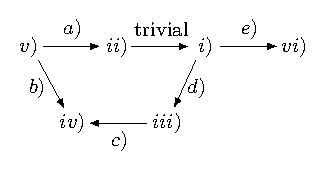
\includegraphics[width=0.5\linewidth]{figures/tikz/proofhopfrinow.pdf}
        \caption{Beweisstruktur für den Satz von Hopf-Rinow}
        \label{fig:proofhopfrinow}
    \end{figure}
\end{bew}<++>

